\documentclass[letterpaper,10pt]{article} 
%% if A4 paper needed, change letterpaper to A4

\usepackage{opticameet3} %% use version 3 for proper copyright statement

%% provide authormark
\newcommand\authormark[1]{\textsuperscript
{#1}}

%% standard packages and arguments should be modified as needed
\usepackage{amsmath,amssymb}
\usepackage[colorlinks=true,bookmarks=false,citecolor=blue,urlcolor=blue]{hyperref} %pdflatex
%\usepackage[breaklinks,colorlinks=true,bookmarks=false,citecolor=blue,urlcolor=blue]{hyperref} %latex w/dvipdf

\begin{document}

\title{Homework 3 Submission}

% \author{Author name(s)}

% \address{Author affiliation and full address}
% \email{e-mail address}
%%Uncomment the following line to override copyright year from the default current year.
%\copyrightyear{2024}

\author{David Wilson \\ Economics 7103 \\ February 5, 2024 }

  
  
\maketitle

\section*{Stata and Python}



\begin{enumerate}
\item Suppose that for a home $i$, you think the underlying relationship between electricity use and predictor variables is $y_i=e^\alpha\delta^{d_i}z_i^{\gamma}e^{\eta_i}$ where $e$ is Euler's number or the base of the natural logarithm, $d_i$ is a binary variable equal to one if home $i$ received the retrofit program, $z_i$ is a vector of the other control variables, and $\eta_i$ is unobserved error, and $\{\alpha,\delta,\gamma\}$ are the parameters to estimate.

\begin{enumerate}
    \item Show that $\ln(y_i)=\alpha+\ln(\delta)d_i+\gamma\ln(z_i)+\eta_i$\\
    Take the natural log of both sides.\\
    \\
        $\ln(y_i)=\ln(e^\alpha\delta^{d_i}z_i^{\gamma}e^{\eta_i})$\\
        $\ln(y_i)=\ln(e^\alpha)+\ln(\delta^{d_i})+\ln(z_i^{\gamma})+\ln(e^{\eta_i})$\\
        $\ln(y_i)=\alpha+d_i\ln(\delta)+\gamma\ln(z_i)+\eta_i$\\
    
    
    \item  What is the intuitive interpretation of $\delta$?\\
    \\
    We could say that $\delta$ is the marginal treatment effect since $d_i$ is the treatment dummy variable. It represents the change in electricity usage if house $i$ received the retrofit program. If the program is expected to lower energy consumption, then we should expect the sign of $\delta$ to be negative.\\
    \\
    \item Show that $\frac{\Delta y_i}{\Delta d_i}=\frac{\delta-1}{\delta^{d_i}}y_i$. What is the intuitive interpretation of $\frac{\Delta y_i}{\Delta d_i}$?\\
    \\
    The intuitive interpretation of $\frac{\Delta y_i}{\Delta d_i}$ that it represents how a change in energy consumption is related to receiving the retrofit program. Since the retrofit program is aimed at reducing monthly energy consumption, it can be hypothesized that $\Delta d_i$ should be negative.\\
    \\
    \item Show that $\frac{\delta y_i}{\delta z_i}=\gamma\frac{y_i}{z_i}$. What is the intuitive interpretation of $\frac{\delta y_i}{\delta z_i}$ when $z_i$ is the size of the home in square feet?\\
    \\
    The intuitive interpretation of $\frac{\delta y_i}{\delta z_i}$ when $z_i$ is the size of the home is that any increase in the size of the home will increase the size of monthly energy consumption.\\
\\
    \item Estimate the log-transformed equation via ordinary least squares on the transformed parameters using any algorithm you would like. Save the coefficient estimates and the average marginal effects estimates of $z_i$ and $d_i$ $\left(\frac{\delta y_i}{\delta z_i}\text{ and }\frac{\Delta y_i}{\Delta d_i}\right)$. Bootstrap the 95\% confidence intervals of the coefficient estimates and the marginal effects estimates using 1000 sampling replications (note that each bootstrap replication should perform both the regression and the second stage calculation of the marginal effect). Display the results in a table with three columns (one for the variable name, one for the coefficient estimate, and one for the marginal effect estimate). Show the 95\% confidence intervals for each estimate under each number.\\
    \\
    \begin{table}[ht]
    \centering
    \begin{threeparttable}
    \caption{Coefficient and Marginal Effect Estimates from Stata}
        \begin{tabular}{l*{2}{c}}
\hline\hline
                    &\multicolumn{1}{c}{Parameter Estimates}&\multicolumn{1}{c}{Marginal Effect Estimates}\\
\hline
Constant            &      -0.769&            \\
                    &[-1.848,0.310]&            \\
Received retrofit   &       0.904&    -110.729\\
                    &[0.893,0.916]&[-130.589,-90.869]\\
Size of home in ft$^2$&       0.894&       0.622\\
                    &[0.880,0.909]&[0.607,0.638]\\
Average outdoor temperature F\textdegree&       0.281&       2.851\\
                    &[0.039,0.524]&[-2.057,7.758]\\
\hline
Observations        &       1,000&       1,000\\
\hline\hline
\end{tabular}

        \begin{tablenotes}\\
          \small  Note: Values in the first column are the coefficient estimates for each variable while the second column displays the average marginal estimates for each coefficient. Both columns have the  95\% confidence interval for each variable in parentheses. 
        \end{tablenotes}
    \end{threeparttable}
\end{table}

    \item  Graph the \textbf{average marginal effects} of outdoor temperature and square feet of the home with bands for their bootstrapped confidence intervals so that they are easy to interpret and compare.\\

    \begin{figure}[ht]\centering
    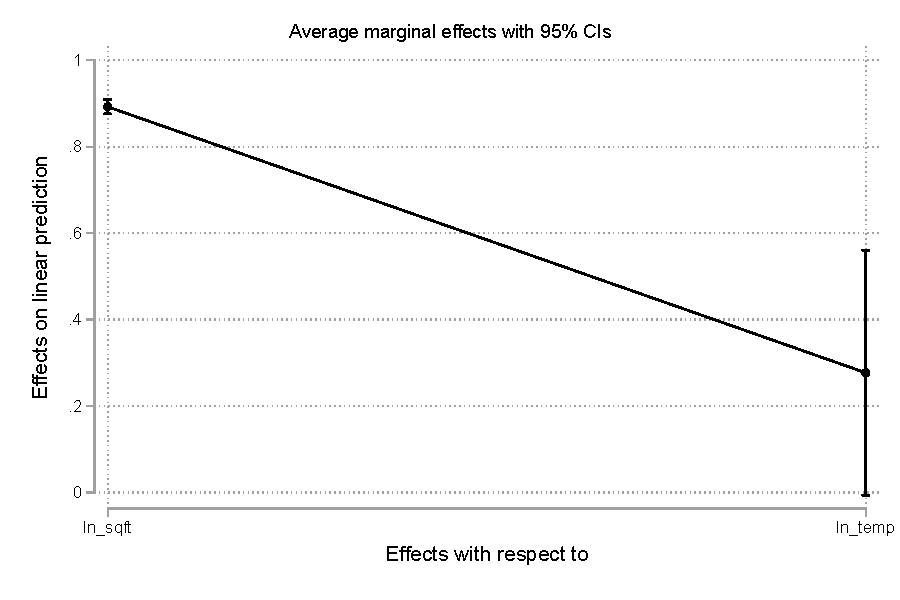
\includegraphics[width=0.7\linewidth]{AME.pdf}
    \caption{This graph shows the average marginal effects of outdoor temperature and the square footage of the home.}
\end{figure}
    




\end{document}